\chapterauthor{Adem Merdzic, Rami Muarrawi, Christopher Schieszler}
\chapter{Einleitung und Projektmanagement}
\label{chap:einleitung}

\section{Ausgangssituation und Motivation}
\label{sec:motivation}
Mobile Robotik und Fahrerassistenzsysteme gehören heute zu den zentralen Anwendungsgebieten der Elektronik und technischen Informatik. Während in industriellen Fahrzeugen hochauflösende 3D-Laserscanner, Radarsysteme und mehrkernige Recheneinheiten zum Einsatz kommen, lassen sich die grundlegenden regelungstechnischen, sensorischen und algorithmischen Prinzipien bereits an einem kompakten Modellfahrzeug im Labor nachvollziehen. Genau hier setzt die schulinterne Projektlinie \emph{Tumbler} an der HTL BULME Graz-Gösting an.

In der vorangegangenen Diplomarbeit des Jahrgangs 2025/26 \cite{Kloeckl2026} wurde bereits ein fahrfähiger Prototyp (\emph{Tumbler~v2}) aufgebaut, der grundlegende Fahrfunktionen und erste Linienfolge-Versuche ermöglichte. Bei der kritischen Bestandsaufnahme dieses Vorgängermodells zu Beginn unseres Projekts zeigten sich jedoch mehrere technische Grenzen, die einen zuverlässigen autonomen Einparkbetrieb im Labor verhinderten:

\begin{itemize}
  \item \textbf{Eingeschränkte Umfelderfassung:} Der Vorgänger nutzte einzelne Ultraschallsensoren mit breiter akustischer Schallkeule. Bei schrägen Hinderniskanten (z.\,B. Begrenzungen einer Parklücke) kam es häufig zu Mehrfachreflexionen und ungenauen Kantenübergängen. Eine lückenlose \qty{360}{\degree}-Rundumsicht war damit nicht erreichbar.
  \item \textbf{Mechanische Engstellen und Wartbarkeit:} Das bisherige 3D-gedruckte Fahrgestell bot zu wenig Einbauraum für eine geordnete Verkabelung. Insbesondere bei gesteckten Dupont-Verbindern, beim Einbau des 2S-Akkupacks sowie beim seitlichen Hauptschalter fehlten definierte Freiräume und Montagepfade.
  \item \textbf{Schaltungstechnische Altlasten:} Auf der älteren Liniensensor-Platine fehlten dokumentierte Dimensionierungen für die IR-Stromversorgung sowie eine definierte Begrenzung der analogen Ausgangsspannung auf den kalibrierten Messbereich des ESP32-S3-ADCs (\qty{2,9}{\volt}). Zudem waren die Anschlüsse über mehrere Einzelstecker verteilt.
  \item \textbf{Software-Struktur:} Eine einfache Hauptschleife (\emph{Super-Loop}) ohne saubere Echtzeit-Trennung zwischen Sensorabfrage, Motorregelung und übergeordneter Fahrlogik stieß bei paralleler Auswertung mehrerer Distanzsensoren rasch an deterministische Grenzen.
\end{itemize}

Aus diesen konkreten Mängeln entstand die Motivation für unser Diplomarbeitsprojekt \emph{Self-Driving Robot Experiments (Tumbler~v3.0)}. Ziel war es nicht, lediglich einzelne Fehler am Bestandsfahrzeug provisorisch auszubessern, sondern eine saubere, nachvollziehbar dokumentierte und mechanisch robuste Plattform zu schaffen, die sowohl selbstständig einparken kann als auch nachfolgenden Jahrgängen als stabile Experimentierbasis dient.

\section{Projektziele und Abgrenzung}
\label{sec:ziele}
Der Funktionsumfang des \emph{Tumbler~v3.0} wurde zu Projektbeginn gemeinsam mit dem Betreuer Prof.~Dipl.-Ing.~Michael Hollegha im Diplomarbeitsantrag festgelegt und gliedert sich in vier Schwerpunkte:

\begin{enumerate}
  \item \textbf{Neukonstruktion der Hardware und Mechanik:} Entwicklung eines 3D-druckbaren, stoßfesten Unibody-Chassis (Revision~v10.0) für den schuleigenen \emph{Bambu Lab P1S}, das alle acht optischen Distanzsensoren, die Hauptplatine, die neu geroutete Liniensensor-Platine, den 2S-Li-Ion-Akkupack, beide Antriebsmotoren sowie den Hauptschalter kollisionsfrei und wartungsfreundlich aufnimmt.
  \item \textbf{360°-Umfelderfassung mittels 8-fach-LiDAR-Array:} Aufbau eines optischen Sensorrings aus acht \emph{VL53L0/1XV2}-Modulen an einem gemeinsamen I\textsuperscript{2}C-Bus mit sequenzieller \gls{xshut}-Adressvergabe, digitaler Messwertfilterung und geometrischer Erkennung von Längsparklücken.
  \item \textbf{Echtzeitfähige Antriebs- und Kursregelung:} Implementierung einer modularen C++-Firmware unter \emph{ESP-IDF} und \emph{FreeRTOS} mit kaskadierter diskreter PID-Drehzahlregelung, Odometrie-Auswertung über Quadratur-Encoder sowie einem zustandsbasierten Einparkautomaten (\gls{fsm}).
  \item \textbf{Verifikation und Reproduzierbarkeit:} Vollständige digitale Absicherung der Mechanik (BRep-Kollisionsprüfung, \qty{25}{\degree}-Sichtkegel-Audit, Montagepfad-Simulation), elektrische Regelprüfungen (ERC/DRC in KiCad) sowie ein strukturierter Labortestplan für das real aufgebaute Fahrzeug.
\end{enumerate}

Bewusst \textbf{abgegrenzt} wurden kamerabasierte Verfahren (Computer Vision / Objekterkennung mittels neuronaler Netze), globale Indoor-Lokalisierungssysteme (UWB, optisches Motion-Capture) sowie der Betrieb im Außenbereich unter direkter Sonneneinstrahlung. Die Infrarot-ToF-Sensoren arbeiten bei \qty{940}{\nano\meter} Wellenlänge und sind für definierte Innenraum- und Laborbedingungen ausgelegt.

\section{Lasten- und Pflichtenheft}
\label{sec:anforderungen}
Um die technischen Teilbereiche eindeutig voneinander abzugrenzen und am Projektende objektiv überprüfen zu können, wurden alle funktionalen und nicht-funktionalen Anforderungen in Tabelle~\ref{tab:anforderungen} mit eindeutigen Kennungen (\texttt{REQ-01} bis \texttt{REQ-20}) und Prioritäten (\textbf{M} = Muss-Kriterium, \textbf{S} = Soll-Kriterium) festgehalten.

\begin{longtable}{@{}p{1.5cm}p{2.3cm}p{8.8cm}c@{}}
\caption{Anforderungskatalog (Lasten- und Pflichtenheft) für den Tumbler~v3.0.}
\label{tab:anforderungen} \\
\toprule
\textbf{ID} & \textbf{Kategorie} & \textbf{Technische Anforderung / Zielwert} & \textbf{Prio} \\
\midrule
\endfirsthead
\toprule
\textbf{ID} & \textbf{Kategorie} & \textbf{Technische Anforderung / Zielwert} & \textbf{Prio} \\
\midrule
\endhead
\bottomrule
\endfoot
REQ-01 & Mechanik & Monolithisches, direkt auf dem Bambu Lab P1S (\qtyproduct{256 x 256}{\milli\meter}) ohne Stützmaterial druckbares Chassis (PLA/PETG, \qty{0,4}{\milli\meter} Düse). & M \\
REQ-02 & Mechanik & Vollständiges Digital Mock-Up (\gls{dmu}) mit \qty{0,000}{\milli\meter\cubed} Volumenkollision zwischen Chassis, Platinen, Sensoren, Steckern, Motoren und Rädern. & M \\
REQ-03 & Mechanik & Mindestens \qty{2,0}{\milli\meter} Restwandstärke um alle Schraubendome; geschlossene Sacklochböden gegen Durchstoßen von Schrauben. & M \\
REQ-04 & Mechanik & Kollisionsfreie Montagepfade für alle 8 LiDAR-Sensoren (inkl. \qty{24}{\milli\meter} Stecker-Freiraum) sowie werkzeugloser Einschub (\emph{Slide-In}) des verlöteten Hauptschalters. & M \\
REQ-05 & Mechanik & Stoßfestigkeit des Front- und Heckbereichs bei einem Aufprall mit \qty{5}{\kilo\meter\per\hour} (\qty{1,39}{\meter\per\second}) mit Sicherheitsfaktor $\mathrm{SF} \ge 3{,}0$. & S \\
REQ-06 & Energie & Spannungsversorgung aus einem 2S-Li-Ion-Akkupack (\qtyrange{6,4}{8,4}{\volt}, \qtyproduct{72 x 39,5 x 19,5}{\milli\meter}) mit mindestens \qty{1,5}{\milli\meter} Einbauspiel umlaufend. & M \\
REQ-07 & Elektronik & Zentraler Mikrocontroller \emph{ESP32-S3-WROOM-1} mit USB-C-Programmier- und Debug-Schnittstelle sowie 10-poligem JST-GH-Anschluss (\texttt{J2}) für den Liniensensor. & M \\
REQ-08 & Elektronik & Sechskanalige Liniensensor-Platine (\qtyproduct{76 x 32}{\milli\meter}) mit \emph{Vishay CNY70}, konstanter IR-Bestromung ($\approx \qty{20}{\milli\ampere}$) und Ausgangsspannung $< \qty{2,9}{\volt}$ (ESP32-S3 ADC1-Grenze). & M \\
REQ-09 & Elektronik & Fehlerfreie Schaltplan- und Layoutprüfung der Liniensensor-Platine (0~ERC-Fehler, 0~DRC-Verletzungen) sowie geprüfte Signal-Netzliste der Hauptplatine Stufe~1. & M \\
REQ-10 & Elektronik & Getrennte Zweikanal-H-Brücken-Ansteuerung (z.\,B. \emph{TB67H450FNG}) für zwei DC-Getriebemotoren \emph{GA37-520} mit Quadratur-Encodern. & M \\
REQ-11 & Sensorik & Lückenlose \qty{360}{\degree}-Umfelderfassung durch acht \emph{VL53L0/1XV2}-Sensoren mit \qty{0}{\percent} Verdeckung der \qty{25}{\degree}-Sichtkegel durch Chassis, Motoren oder Räder. & M \\
REQ-12 & Sensorik & Sequenzielle \gls{xshut}-Initialisierung und eindeutige dynamische I\textsuperscript{2}C-Adressvergabe (\texttt{0x30} bis \texttt{0x37}) ohne Buskonflikte bei Systemstart. & M \\
REQ-13 & Sensorik & Messwertfilterung (Median- und EMA-Filter) zur Unterdrückung von Einzel-Ausreißern und Behandlung ungültiger Messwerte ($\ge \qty{8190}{\milli\meter}$ bzw. Timeout). & M \\
REQ-14 & Sensorik & Geometrische Erkennung von Längsparklücken ab einer Mindestlänge von $L_{\mathrm{L\ddot{u}cke}} \ge \qty{410}{\milli\meter}$ und Tiefe $D_{\mathrm{L\ddot{u}cke}} \ge \qty{210}{\milli\meter}$ während der Vorbeifahrt. & M \\
REQ-15 & Software & Modulare C++-Firmware unter \emph{ESP-IDF} mit \emph{FreeRTOS}-Tasks und klarer Trennung von Sensorik, Regelung und Zustandsautomat. & M \\
REQ-16 & Regelung & Diskrete PID-Drehzahlregelung beider Antriebsräder mit \qty{100}{\hertz} Abtastrate ($T_s = \qty{10}{\milli\second}$) und \emph{Clamping Anti-Windup} gegen Integrator-Sättigung. & M \\
REQ-17 & Regelung & Autonomes Spurfolgen auf einer kontrastreichen schwarzen Linie (\qtyrange{15}{25}{\milli\meter} Breite) mittels gewichteter Schwerpunktberechnung der 6 CNY70-Kanäle. & M \\
REQ-18 & Autonomie & Deterministischer Einpark-Zustandsautomat (\gls{fsm}) mit automatischer Rückwärts-S-Kurve, Ausrichtung in der Parklücke und Kollisionsabbruch bei $d < \qty{60}{\milli\meter}$. & M \\
REQ-19 & Sicherheit & Hardwareseitiger Hauptschalter in der Batteriezuleitung sowie softwareseitiger Watchdog und Not-Aus bei Sensor-Timeout oder Blockierstrom. & M \\
REQ-20 & Doku & Nachvollziehbare Gesamtdokumentation nach HTL-BULME-Standard mit vollständiger Stückliste, Pinbelegung, CAD-/PCB-Nachweisen und Labortestplan. & M \\
\end{longtable}

\section{Projektmanagement und Teamorganisation}
\label{sec:projektmanagement}
Ein 3-Personen-Projekt über ein gesamtes Schuljahr erfordert klare Zuständigkeiten, damit Hardware, Mechanik und Software parallel entstehen können, ohne sich gegenseitig zu blockieren.

\subsection{Teamstruktur und Arbeitspakete}
Die Aufgaben wurden entlang der fachlichen Schwerpunkte auf die drei Projektmitglieder aufgeteilt (Tabelle~\ref{tab:team}). Übergreifende Themen wie die Systemarchitektur, Schnittstellen-Definitionen (Pinbelegung, Koordinatensysteme) und die finale Systemintegration wurden gemeinsam bearbeitet.

\begin{table}[htbp]
\centering
\caption{Teamzusammensetzung und fachliche Verantwortungsbereiche.}
\label{tab:team}
\begin{tabular}{@{}p{3.6cm}p{4.4cm}p{6.2cm}@{}}
\toprule
\textbf{Teammitglied} & \textbf{Hauptverantwortung} & \textbf{Zugeordnete Arbeitspakete} \\
\midrule
\textbf{Christopher Schieszler} & Hardware, Schaltungstechnik, PCB-Design \& Mechanik/CAD & AP2 (Liniensensor-PCB R2), AP3 (Hauptplatine Stufe 1/2), AP4 (Unibody-Chassis v1–v10, DMU \& 3D-Druck) \\
\textbf{Rami Muarrawi} & Sensorik, I\textsuperscript{2}C-Multiplexing \& Umfelderkennung & AP4 (CAD-Integration LiDAR-Pods), AP5 (8× VL53L0X XSHUT-Treiber \& Filterung), AP6 (Parklücken- \& Linienerkennung) \\
\textbf{Adem Merdzic} & Embedded Software, Regelungstechnik \& Autonomie & AP7 (FreeRTOS-Architektur, Odometrie \& PID-Regler), AP8 (Einpark-FSM, Safety \& Gesamtsystem-Integration) \\
\midrule
\textbf{Prof.~Dipl.-Ing.~M.~Hollegha} & Diplomarbeitsbetreuer & Fachliche Begleitung, Meilenstein-Reviews, Laborfreigabe \\
\bottomrule
\end{tabular}
\end{table}

\subsection{Zeitplan und Meilensteine}
Die zeitliche Abfolge der neun Arbeitspakete (AP1 bis AP9) sowie der sechs verbindlichen Meilensteine (M1 bis M6) ist im Gantt-Diagramm in Abbildung~\ref{fig:gantt} dargestellt. Tabelle~\ref{tab:meilensteine} fasst die zugehörigen Lieferergebnisse (\emph{Deliverables}) zusammen.

\begin{figure}[htbp]
  \centering
  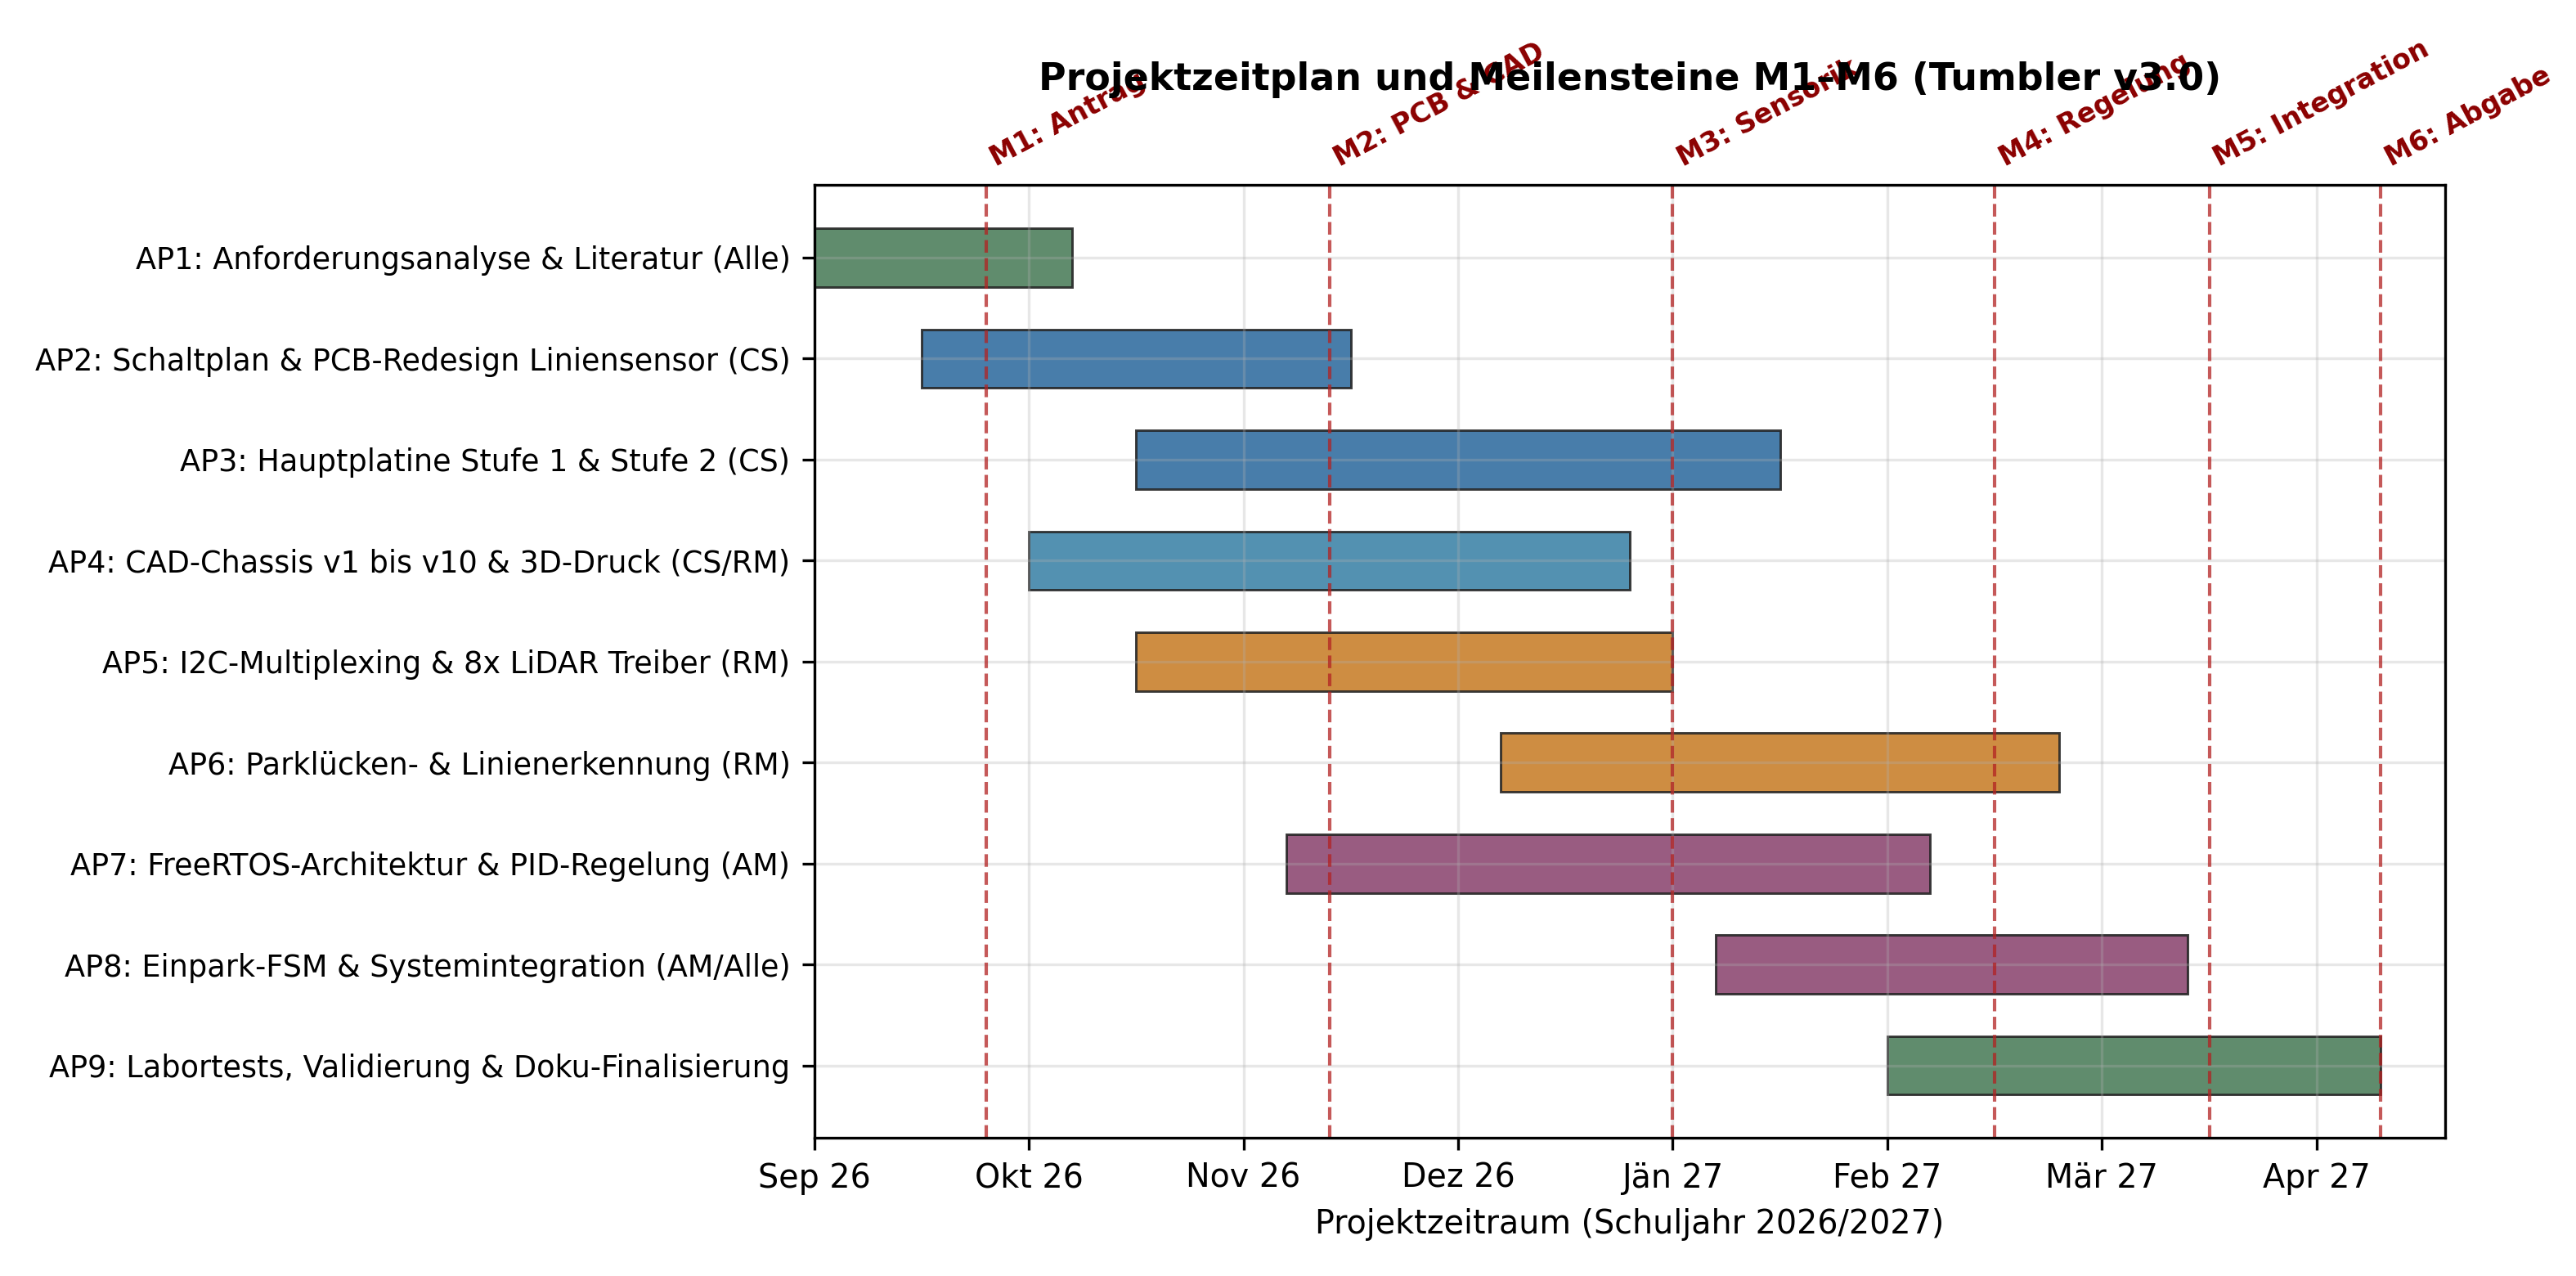
\includegraphics[width=0.98\textwidth]{figures/fig_gantt_milestones.png}
  \caption{Projektzeitplan (Gantt-Diagramm) mit Arbeitspaketen AP1--AP9 und Meilensteinen M1--M6.}
  \label{fig:gantt}
\end{figure}

\begin{table}[htbp]
\centering
\caption{Meilensteinplan M1--M6 gemäß Projektantrag.}
\label{tab:meilensteine}
\begin{tabular}{@{}p{1.2cm}p{2.2cm}p{3.6cm}p{7.2cm}@{}}
\toprule
\textbf{Nr.} & \textbf{Zieltermin} & \textbf{Meilenstein} & \textbf{Abnahmekriterium / Ergebnis} \\
\midrule
M1 & Okt. 2026 & Projektantrag \& Konzept & Freigegebener ABA-Antrag, Lastenheft, Systemarchitektur, Git-Repository eingerichtet. \\
M2 & Nov. 2026 & PCB \& CAD-Freeze & Fehlerfreie Liniensensor-Platine R2 (ERC/DRC = 0), Hauptplatine Stufe 1 geprüft, Chassis v10.0 druckfertig (Watertight STL). \\
M3 & Jän. 2027 & Sensorik-Inbetriebnahme & Alle 8 LiDAR-Sensoren stabil am I\textsuperscript{2}C-Bus (\texttt{0x30}--\texttt{0x37}), CNY70-Kalibrierung im Labor verifiziert. \\
M4 & Feb. 2027 & Regelung \& Spurfolge & Kaskadierter PID-Regler auf dem Fahrzeug abgestimmt, reproduzierbare Linienverfolgung. \\
M5 & Mär. 2027 & Autonomes Einparken & Vollständiger Parkzyklus (Suchen, Vermessen, Rückwärts-Einparken, Stopp) am Testparcours. \\
M6 & Apr. 2027 & Abgabe \& Präsentation & Gebundene Diplomarbeit, Poster, lauffähiger Demonstrator zur Reife- und Diplomprüfung. \\
\bottomrule
\end{tabular}
\end{table}

\subsection{Risikoanalyse und Gegenmaßnahmen}
Bereits in der Konzeptphase wurden die größten technischen und organisatorischen Risiken bewertet (Eintrittswahrscheinlichkeit $W \in \{1..5\}$, Auswirkung $A \in \{1..5\}$, Risikoprioritätszahl $\mathrm{RPZ} = W \cdot A$). Tabelle~\ref{tab:risiko} dokumentiert die abgeleiteten Maßnahmen.

\begin{table}[htbp]
\centering
\caption{Projekt-Risikoanalyse mit konkreten technischen Gegenmaßnahmen.}
\label{tab:risiko}
\begin{tabular}{@{}p{0.9cm}p{3.4cm}ccc p{7.0cm}@{}}
\toprule
\textbf{ID} & \textbf{Risiko} & \textbf{W} & \textbf{A} & \textbf{RPZ} & \textbf{Umgesetzte Gegenmaßnahme} \\
\midrule
R1 & I\textsuperscript{2}C-Buskonflikte oder Blockade bei 8 Sensoren & 4 & 4 & 16 & Sequenzielle \gls{xshut}-Initialisierung mit Hi-Z-Freigabe, \qty{500}{\milli\second} Software-Timeout und sauberer Bus-Pull-up-Auslegung. \\
R2 & Mechanische Kollisionen / unpassender 3D-Druck & 4 & 4 & 16 & Vollständiges 127-Körper-\gls{dmu} mit automatisierter BRep-Kollisionsprüfung (\qty{0,000}{\milli\meter\cubed}), Montagepfad-Checks und Watertight-STL-Test vor dem Druck. \\
R3 & Störeinkopplung der DC-Motoren auf CNY70 / ADC & 3 & 4 & 12 & Durchgehende GND-Fläche, getrennte Masseführung für LED-Stromsenken, \qty{10}{\nano\farad}-RC-Tiefpass je Kanal ($f_g = \qty{1,93}{\kilo\hertz}$) und \qty{100}{\ohm}-Serienwiderstände. \\
R4 & Überschreitung der ADC1-Grenze (\qty{2,9}{\volt}) & 2 & 4 & 8 & Auslegung des Ausgangs-Spannungsteilers (\qty{10}{\kilo\ohm} / \qty{47}{\kilo\ohm}) auf nominal \qty{2,72}{\volt} (Worst-Case \qty{2,87}{\volt} $< \qty{2,9}{\volt}$). \\
R5 & Lieferverzögerungen bei Platinen / Bauteilen & 3 & 3 & 9 & Frühzeitige Standardbauteil-Wahl (0805/1206, gängige MPNs) und Aufbau eines 4-Sensor-Breadboard-Prüfstands für parallele Firmware-Entwicklung. \\
\bottomrule
\end{tabular}
\end{table}

\subsection{Versionsverwaltung und Git-Workflow}
Sämtliche Projektdateien (KiCad-Schaltpläne, CAD-Modelle, ESP-IDF-Quellcode und diese LaTeX-Diplomarbeit) werden zentral im GitHub-Repository \texttt{chrisitrisi/SelfDrivingRobotExperiments} verwaltet. Um Merge-Konflikte zwischen binären CAD-/PCB-Dateien und Textquellen zu vermeiden, arbeiten wir mit dedizierten Themen-Branches:

\begin{itemize}
  \item \texttt{3D\_Design}: Parametrische Python-CAD-Skripte, STEP-/STL-Fertigungsdateien und DMU-Vorschaubilder (aktueller Stand: Revision~v10.0).
  \item \texttt{PCB}: KiCad-Projekte für den Liniensensor (\texttt{Liniensensor\_Redesign}) sowie die Hauptplatine (\texttt{Tumbler\_Stage1}), Gerber-Daten, Stücklisten und ERC-/DRC-Berichte.
  \item \texttt{Main\_code}: ESP-IDF-Firmware-Projekt in C++ inklusive der Portierung der \emph{VL53L0X}-Komponente.
  \item \texttt{Dokumentation}: LaTeX-Quellen, Abbildungen, Literaturdatenbank, Antrag und Präsentationsunterlagen.
\end{itemize}

In der Praxis zeigte sich bei großen Projektarchiven (über \qty{100}{\mebi\byte} bei gepackten ZIP-Dateien), dass GitHub entsprechende Pushes ablehnt. Durch eine gezielte \texttt{.gitignore}-Konfiguration für komprimierte Archive (\texttt{*.zip}, \texttt{*.7z}) und temporäre LaTeX-Hilfsdateien (\texttt{*.aux}, \texttt{*.log}, \texttt{*.toc}) bleibt das Repository schlank und jederzeit reproduzierbar synchronisierbar.
